\documentclass[12pt,dvipdfmx]{book}
\usepackage{otf}

\topmargin=-10mm
\headheight=12pt
\headsep=0mm
\textheight=245mm
\oddsidemargin=-5mm
\evensidemargin=-5mm
\textwidth=170mm

\usepackage[style=phys,articletitle=false,%
biblabel=brackets,chaptertitle=false,pageranges=false,%
backend=bibtex]{biblatex}
\DeclarePrefChars{'-}
\addbibresource{../../library.bib}

\usepackage{todonotes}
\renewcommand{\baselinestretch}{2}
\usepackage{tikz}
%\usepackage{mediabb}
\usepackage{subcaption}
\usepackage{amsmath,amsfonts,amsthm,amssymb}
\usepackage{ascmac}
\usepackage{algorithm}
\usepackage{algorithmic}
\usepackage{graphicx}
\usepackage{color}
\usepackage{dcolumn}
\usepackage{bm}
\usepackage{book tabs}
\usepackage{braket}
\usepackage{setspace}
\usepackage{docmute}
\usepackage{listings}
\usepackage[colorlinks]{hyperref}
%\newcommand{\figref}[2][{}]{\hyperref[#2]{\figurename~\ref{#2}#1}}

\theoremstyle{definition}
\newtheorem{definition}{Definition}[section]
\newtheorem{theorem}{Theorem}[section]
\newtheorem{corollary}{Corollary}[theorem]
\newtheorem{lemma}[theorem]{Lemma}

\newcounter{one}
\setcounter{one}{1}

\pagestyle{plain}

\begin{document}

\title{Effects of Boundary Conditions on Magnetic Friction}
\author{Kentaro Sugimoto \\ Department of Physics, The University of Tokyo }
\date{\today}
\maketitle
Acknowledgement.

\clearpage
\begin{center}
\large{{\bf Abstract}}
\end{center}
In the present thesis, hogehoge.
Moreover, fugafuga.
\listoftodos
\tableofcontents
% !TeX root = Body.tex
\chapter{Introduction}
%The system is one of the simplest model of two-dimensional magnetic friction. Its spatial and spin dimensionality are far from realistic materials around us. However, we can use several facts from the exact solution for the two-dimensional Ising model, which makes the analysis easier than higher-dimensional cases.
The sliding friction in solids is a too complex problem to deal with, despite the fact that our daily lives are linked with it in various forms. One reason is that there is no general theory for various and a number of physical degrees of freedom, which determines the most important degree for the sliding friction as a phenomenon.

One may think that, with the skill of statistical mechanics, we can deal with the problem in a systematic manner. But there still remains several problems as follows:
\begin{itemize}
	\item \textbf{Problem1}: The sliding friction is essentially non-equilibrium phenomenon.
	\item \textbf{Problem2}: We cannot directly observe the sliding surface.
\end{itemize}

In this chapter we introduce two of the most famous problems with dealing the frictional force as the problem of statistical mechanics. We give recent developments for solving these problems. We then propose the question related to a problem about the \textit{manipulation} of the sliding friction which occurs in highly lubricated solids. To this end we simplify the problem into a dimensional crossover in lattice systems.

\section{Sliding Frictions as Non-Equilibrium Problems}
We can regard the sliding friction as follows in an elementary manner. We consider an object $O$ and a substrate $S$, and let $S$ slide against $O$ with them contacting and an external force. When $O$ and $S$ interact with each other, the kinetic energy of $O$ given by the external force is expected to lose by the interaction, and then the entire system $O+S$ heats up (if they form a closed system) or an energy dissipation occurs from the system to external environment (if they form an open system). In the latter case, under the assumption that the dissipation process stationarily occurs, the frictional force $f_{\rm fric}$ take a constant value balancing with the external force. This setup is realized when we keep the external force $f_{\rm ext}$ so that the sliding velocity $v$ take a constant value. Then the frictional force $f_{\rm fric}$ is dealt with as a function of the sliding velocity as $f_{\rm fric}=f_{\rm fric}(v)$.

The traditional way of statistical mechanics, called the linear response theory, appears to deal with the problem under the condition that the velocity $v$ is much smaller than the rate $\xi/\tau$, where $\xi$ and $\tau$ are the characteristic length and time of the system. But we already know well the phenomenon that the static frictional force is non-zero value for several systems. In such systems, we easily observe the non-linearity of the frictional force $f_{\rm fric}$ for the velocity $v$. This simply shows us the complexity of the problem which cannot be captured by applying the traditional way.

Many researches have dealt with the problem using the numerical way or limiting to an extreme region of parameters to avoid attack with the perturbative way.

\section{Impossibility of the Observation of the Sliding Surface}
The dimensionality of the sliding surface is up to two-dimension, if that of the whole system is the three-dimension. Sliding surfaces of such systems are different in many ways from well-known two-dimensional surfaces of three-dimensional solids which have investigated for many years, then we cannot perform a direct observation of the sliding surface by apparatuses such as microscopes. The difficulty prevents us from revealing non-equilibrium properties of the sliding friction.

There is the way to observe the contact plane with the microscope and an optically transparent matter, but most researches avoid a direct observations by measuring other observables to indirectly observe the contact plane.

\section{Manipulating the Friction}

Recent researches well revealed the nature of sliding frictions. This also leads us to conflict with a new problems about the friction in atomically microscopic systems.

Ordinary frictions in solids are mostly governed by excitations of phonon degrees of freedom, because the contact plane is almost always rough than the scale of the atom. But once we get the contact plane highly lubricated, other degrees of freedom, such as the orbital and the spin of electrons, emerges as the main contribution to the friction, in addition to the phonon excitation. 

We are already familiar with the most remarkable example of such a system in our daily lives, which is called \textit{micro electric mechanical system} (\textbf{MEMS}). MEMS plays an important role in the head of inkjet printers, the accelerometer in smartphones and so on. As an aspect of the MEMS, there are processed planes with an accuracy of a micrometer or a nanometer and they are also moving parts. Thus they inevitably experience the new type of the friction by operations. In addition the smaller size of these systems makes the problem more serious, because the rate of the surface area over the volume of a system become larger with the smaller size in general.

Thus we have to tackle with the issue of manipulation the friction in such a smaller system by getting more fundamental knowledges of the friction.

\section{Magnetic Friction}
The way to manipulate the friction in such a small system is less understood than its nature. Thus we consider the manipulation of magnetic materials as an easier problem to analyze by lattice models and its simulations. 

Frictions in such models themselves are a new type of the problem problems, and date back to the numerical research by Kadau et al.\cite{Kadau2008}. They have revealed that two square lattices of a Ising model which slide with each other experience the friction, depending on the temperature and the sliding velocity, by Monte Carlo simulations. Immediately after the research, it was revealed that the Ising model goes to a non-trivial non-equilibrium phase transitions (\textbf{NEPT}) in the high-velocity limit, where the two sliding models are decoupled in terms of the correlation between the two models and feel a mean field depending the magnetization of each other\cite{Hucht2009b}. By this treatment, we are able to access the novel critical point which is located in a higher temperature than the ordinal critical point in general for models with arbitrary dimensions and geometries (see Chapter \ref{ch:review}). In addition to the results, they developed a new algorithm which enables the analytical treatment in more detail and revealed the non-equilibrium critical point for arbitrary velocities. 

Based on their results\cite{Hucht2009b}, we consider a dimensional crossover from one-dimension to two in Ising models with two fixed boundary conditions. In the one-dimensional limit the boundary conditions seem to have the most effect on the friction, whereas in the two-dimensional limit there seems to be no effects. Behaviors in the both limits for the free boundary condition correspond to the results\cite{Hucht2009b}. In this way we think the problem of the manipulation as the dimensionality with different boundary conditions. Simpler boundary conditions would be realized by experiments with the boundary spins of relatively moving magnets aligned.
% !TeX root = Body.tex

\chapter{Velocity-driven Non-equilibrium Phase Transition in Ising Models}\label{ch:review}

To discuss the non-equilibrium crossover between two different dimensions, we have to make a brief review the exact results\cite{Hucht2009b} by Hucht. Their analysis is based on the fact that two Ising cylinders with relative motion make a novel mean field and they lead the system to non-trivial phase transition.

We now consider two equivalent square lattices of Ising model each of which contacts with the other by one of its one-dimensional boundary. If we leave two models alone, we can regard the models as an Ising model with a twice the size. With the coupling to the heat bath, we expect the model thermalize. But one of the couple are moving along the contact plane with a constant velocity $v$, the entire model goes into a non-equilibrium stationary state, instead of thermalization. The non-equilibrium stationary state well describes the behavior of two magnetic materials are sliding with the friction. This setup are explained in detail in Chapter \ref{chap:NumSim}.

The two dimensional Ising model has the phase transition which occurs at the critical temperature $T_{\rm c}=\text{\textcolor{red}{exact value or equation form}}$ in the thermodynamical limit $N/V\to\infty$ with $N/V=\text{const.}$, where $N$ is the number of spins and $V$ is the volume of the system as a well known fact. The model which we consider in this chapter is no exception, if the sliding velocity $v$ is set to zero. The result\cite{Hucht2009b} claims that the critical temperature $T_{\rm c}$ \textit{branches} at the point $v=0$ towards the limit $v=\infty$. The system exhibits the ordinary phase transition at the vertical line $T=T_{\rm c}(v=0)$, whereas exhibits a novel phase transition at the curve $T=T_{\rm c}(v>0)$ where the magnetization grows up near the contact plane rather than the rest \textcolor{red}{cite the phase diagram of the ref.}. These phenomena were first reported in the numerical results\cite{Kadau2008} by Kadau et al. using Monte Carlo simulations with both Metropolis algorithms and Glauber algorithms in two-dimensional models, and then investigated in more exact manner\cite{Hucht2009b} by Hucht in several dimensions and model geometries. One of the important point in the latter result is that for $v\to 0$ we can write the closed exact equation for the \textit{second} critical temperature $T_{\rm c}(v>0)$. In addition it is also important that a novel algorithm, called \textit{multipricative rate}, enabled us to give the equation for $T_{\rm c}(v>0)$ which fully depends on the algorithm for arbitrary $v>0$.

If the velocity $v$ is much less than the rate $\xi^{(\rm eq)}_{x}(\beta)/\tau^{(\rm eq)}_{x}(\beta)$, we can expect the system to behave well similarly to its equilibrium state. We denote the correlation length along the direction parallel to the contact plane by $\xi^{(\rm eq)}_{x}(\beta)$ and the correlation time by $\tau^{(\rm eq)}_{x}(\beta)$ respectively for the equilibrium state of an inverse temperature $\beta:=(k_{\rm B}T)^{-1}$. This corresponds to the circumstance that the pumped energy by the constant sliding is most quickly relaxed towards the heat bath. In the case, the structure of domain walls near the contact plane is well sustained. On the other hand, the velocity $v$ much greater than the rate $\xi^{(\rm eq)}_{x}(\beta)/\tau^{(\rm eq)}_{x}(\beta)$ will lead the system to a stationary state much far from equilibrium, then the structure near the contact plane will be destroyed. 

In the latter case that the velocity is much higher, a mean field picture that two sets of the moving spins along the contact plane act on the other \textit{relatively} moving spins as the spatially-averaged effective field. In other words, the magnetization of one half of the system corresponds the effective field of the other, and vice versa. This enables us to write a self-consistent equation for the temperature $T_{\rm c}(v\to\infty)$.

We summarize the result for one-dimensional chains and that of two-dimensional planes, in order to discuss the crossover from one-dimension to two-dimension in our models in Chapter \ref{chap:Summary}.

\textcolor{red}{Brief review.}
% !TeX root = Body.tex
\chapter{Numerical Simulations}\label{chap:NumSim}

\section{Setup of the Model}\label{sec:SetupModel}
Sliding friction is a form of energy dissipation on the surface between a moving object and its substrate. The dissipated energy is originated in the kinetic energy of the moving object. We here consider a constantly moving case in which an external force maintains the motion of the object with endless supply of its kinetic energy. This view leads to its \textit{non-equilibrium stationary state}. When the system is in a non-equilibrium stationary state, it is often easy to calculate \textit{energy currents} such as the frictional heat, its power and so on. Applying the view to our case in which two square lattices of the Ising model slide against each other, we can formulate the problem as follows; see Fig.~\ref{fig:CutIsing}.
\begin{enumerate}
	\item We prepare a square lattice of the Ising model of size $L_{x}\times L_{z}$ and impose periodic boundary conditions in the transverse ($x$) direction. We first set the system in the equilibrium state of a temperature $T$, whereas we set the open boundary conditions in the longitudinal ($z$) direction for the moment.
	\item We cut the system along the $x$-direction into two parts, maintaining interactions on the cut.
	\item We slide two parts along the cut plane with relative velocity $v$. In other words, we shift the upper half by a lattice constant every $1/v$ unit time. 
\end{enumerate}

\begin{figure}[htbp]
	\centering
	\includegraphics[width=0.25\linewidth]{../../Slides/Ingredients/03-CutIsing.pdf}
	\caption{Two cylinders of the Ising model sliding with the velocity $v$.}
	\label{fig:CutIsing}
\end{figure}

The Hamiltonian of the system is given by
\begin{align}
&\hat{H}=\hat{H}_{\rm upper} + \hat{H}_{\rm lower} + \hat{H}_{\rm slip}(t),
\end{align}
where
\begin{align}
&\hat{H}_{\rm upper}:=-J\sum_{\langle i,j\rangle\in\mathrm{upper}}\hat{\sigma}_{i}\hat{\sigma}_{j}\label{ham:upper}, \\
&\hat{H}_{\rm lower}:=-J\sum_{\langle i,j\rangle\in\mathrm{lower}}\hat{\sigma}_{i}\hat{\sigma}_{j}\label{ham:lower}, \\
&\hat{H}_{\rm slip}(t):=-J\sum_{\langle i,j(t)\rangle\in\mathrm{slip}}\hat{\sigma}_{i}\hat{\sigma}_{j(t)}\label{ham:slip}
\end{align}
upper, lower and slip representing the set of interacting spin pairs on the upper half, the lower half and the slip plane, respectively.
Shift operations lead the system to repeated \textit{pumping} and \textit{dissipation} processes as follows:
\begin{enumerate}
	\item \textbf{Shift}: A shift operation excites the energy on the slip plane by the amount $\langle\hat{H}_{\rm slip}(t')-\hat{H}_{\rm slip}(t)\rangle_{\rm st}$. The letter $t'$ denotes the time just after the shift operation at time $t$.
	\item \textbf{Relax-1}: The excited energy on the slip plane $\langle\hat{H}_{\rm slip}(t')-\hat{H}_{\rm slip}(t)\rangle_{\rm st}$ dissipates to the entire system.
	\item \textbf{Relax-2}: The excited entire system relaxes towards the equilibrium.
\end{enumerate}
We defined the stationary state average $\langle\hat{A}\rangle_{\rm st}:=\sum_{i}A_{i}p^{(\rm st)}_{i}$ for an arbitrary observable $\hat{A}$, where $\{A\}_{i}$ are eigenvalues of $\hat{A}$ and $\{p^{(\rm st)}_{i}\}$ is the stationary-state probability distribution, which is different from the equilibrium (canonical) probability distribution $p^{(\rm eq)}_{i}\propto\exp\left[-E_{i}/k_{\rm B} T\right]$. Note that the distribution $\{p^{(\rm st)}_{i}\}$ depends on the sliding velocity $v$. 

The excited and relaxed amounts of energy per unit time correspond to the energy pumping and dissipation, respectively. The energy pumping $P(t)$ and dissipation $D(t)$ are given by
\begin{align}
P(t):=&\sum_{i_{v}=0}^{v-1}\left\langle \hat{H}_{\rm slip}\left(t'-1+\frac{i_{v}}{v}\right) - \hat{H}_{\rm slip}\left(t-1+\frac{i_{v}}{v}\right)\right\rangle_{\rm st},\\
D(t):=&\sum_{i_{v}=0}^{v-1}\left\langle \hat{H}_{\rm slip}\left(t-1+\frac{i_{v}+1}{v}\right) - \hat{H}_{\rm slip}\left(t'-1+\frac{i_{v}}{v}\right)\right\rangle_{\rm st},
\end{align}
respectively. $P(t)$ and $D(t)$ correspond to the energy difference due to the \textbf{Shift} and the \textbf{Relax} processed, respectively. Note that absolute values of $P(t)$ and $D(t)$ become equal to each other in the non-equilibrium stationary state, by its definition.

\section{Definitions of Physical Quantities}
We now consider the case in which the system is in a non-equilibrium stationary state. We denote by $P(L_{x}, L_{z}, T)$ and $D(L_{x}, L_{z}, T)$ the long-time limit of energy pumping $P(t)$ and dissipation $D(t)$ for a system of size $L_{x}\times L_{z}$ at the temperature $T$. We define the frictional force density $f(L_{z}, T)$ by
\begin{align}
f(L_{z}, T):=\lim_{L_{x}\to\infty}\frac{F(L_{x}, L_{z}, T)}{L_{x}}.
\end{align}

In numerical simulations, we calculate the frictional force $F(L_{x}, L_{z}, T)$ using its power $D(L_{x}, L_{z}, T)$ by the formula
\begin{align}
F(L_{x}, L_{z}, T)=\frac{D(L_{x}, L_{z}, T)}{v}\label{for:frictionalforce}.
\end{align}

We can easily verify the formula \eqref{for:frictionalforce} by considering general cases in which the frictional force and its power are both time dependent. Denoting the frictional force $F(x)$ at the position $x$, it holds that
\begin{align}
\int_{t_{0}}^{t_{1}}dt\;D(t)=\int_{x(t_{0})}^{x(t_{1})}dx\;F(x)=\int_{t_{0}}^{t_{1}}\frac{dx}{dt}dt\;F(x(t))=v\int_{t_{0}}^{t_{1}}dt\;F(x(t))\label{rel:PowerFrictionalforce}
\end{align}
for a time dependent $D(t)$, because $dx/dt=v$. Under the assumption of a non-equilibrium stationary state, the integrands in both-hand sides of the relation \eqref{rel:PowerFrictionalforce} are still equal to each other in the long-time limit, and hence 
\begin{align}
D(L_{x}, L_{z}, T)=vF(L_{x}, L_{z}, T).
\end{align}
From now we call the quantity $D(L_{x}, L_{z}, T)$ the \textit{energy dissipation}.

Our model always reaches a non-equilibrium stationary states in the long-time limit $t\to\infty$, which depends on the temperature $T$ and the sliding velocity $v$; We will prove it in .~\ref{chap:ProofEx}. We use the fact that $\lim_{t\to\infty}|D(t)|=\lim_{t\to\infty}|P(t)|$ in order to estimate the average $\bar{D}$; the average $\bar{P}$ has less statistical fluctuation~\cite{Magiera2009a, Magiera2011, Magiera2011b}. We therefore have
\begin{align}
P(L_{x}, L_{z}, T)=vF(L_{x}, L_{z}, T)\label{for:frictionalforce2}.
\end{align}
We also define the bulk energy density $\epsilon_{\rm b}(L_{z}, T)$ as follows:
\begin{align}
\epsilon_{\rm b}(L_{z}, T):=\lim_{L_{x}\to\infty}\frac{E_{\rm b}(L_{x}, L_{z}, T)}{L_{x}L_{z}},
\end{align}
where $E_{\rm b}(L_{x}, L_{z}, T)$ is the energy of the entire system. From this, we define the bulk heat capacity $c_{\rm b}(L_{z}, T)$ as follows:
\begin{align}
c_{\rm b}(L_{z}, T):=\frac{\partial \epsilon_{\rm b}(L_{z}, T)}{\partial T}.
\end{align}

\section{Non-equilibrium Monte Carlo Simulation}
The dissipation process towards the heat bath occurs via a spin flip. This fundamental processes do not only describe equilibrium states but also non-equilibrium stationary states at a fixed temperature $T$~\cite{Glauber1963}. Using Monte Carlo method, we simulate this process.

\subsection{Introduction the Time Scale to Ising Models}
In order to calculate dynamical observables such as the frictional power \eqref{for:frictionalforce2} and its dissipation rate \eqref{for:frictionalforce}, we have to define \textit{a unit time} for finite size systems. 

For the equilibrium Monte Carlo simulation, the most naive approach for the equilibrium state is the single-spin-flip algorithm, where we perform the sequence of a random selection of a spin and its flip with a temperature dependent probability $p(T)$. Whatever we use as the probability for the Monte Caro simulation should satisfy a good property, called \textit{detailed balanced condition}, which certainly leads the system towards the true equilibrium state with enough repetition of the sequence. For example, we often use the Metropolis probability $p_{\rm M}(T):=\min\{1,\mathrm{e}^{-\frac{\Delta E}{k_{\rm B}T}}\}$ as the probability $p(T)$, where $\Delta E$ is the energy difference due to the flip. We often call a \textit{Monte Carlo step} a single process of the algorithm, and define a \textit{Monte Carlo sweep} by $N$ Monte Carlo steps, where $N$ is the number of spins.

Which do we have to define a unit time by a Monte Carlo step or a Monte Carlo sweep? Its answer can be seen in the following manner: We often assume that a statistical mechanical model are coupling to a heat bath by each local degree of freedom. The temperature of the system is kept constant by the heat bath and exchanges its energy with the heat bath through local degrees of freedom. It is most natural to assume that the frequency of the exchanging process is dependent only on the temperature of the heat bath. Thus the total number of times exchanged are proportional to the number of degrees of freedom of the system. It is justified to define a unit time by a Monte Carlo sweep. Note that the more spins the system contains, the higher time resolution we can simulate with.

\subsection{Slip Plane with the Velocity $v$}
Using the introduced time scale, we can also introduce the slip plane with the velocity $v$ to the system with $N$ spins. Corresponding to the setup in Sec.~\ref{sec:SetupModel}, we perform an extended single-spin-flip algorithm as follows:
\begin{enumerate}
	\item \textbf{Shift}: We shift the upper half of the lattice by a lattice constant.
	\item \textbf{Flip}: We perform ordinary single flips for $N/v$ times.
	\item We repeat the processes 1 and 2 for $v$ times.
\end{enumerate}
In the extended algorithm, the upper half slides with the velocity $v$ in a unit time at regular intervals. We proved the fact that this algorithm leads the system of any size to a non-equilibrium stationary state depending on the temperature $T$ and the velocity $v$ (see App.~\ref{chap:ProofEx} for details).

\subsection{Calculation Method}
The observables that we are interested in are the frictional power $P(t)$ and its dissipation rate $D(t)$. In Monte Carlo simulations, they are the energy difference for a unit time due to the shift and the flip operation, respectively. Both observables have the same absolute value in the long-time limit.


%\chapter{Numerical Simulations}

\section{Definitions of Physical Quantities}

From now we consider the case that the system is in a non-equilibrium steady state. We define frictional force density $f_{\mathcal{B}}(L_{z}, T)$ by
\begin{align}
f_{\mathcal{B}}(L_{z}, T):=\lim_{L_{x}\to\infty}\frac{F_{\mathcal{B}}(L_{x}, L_{z}, T)}{L_{x}},
\end{align}
where $F_{\mathcal{B}}(L_{x}, L_{z}, T)$ is the frictional force of a system with a size $L_{x}\times L_{z}$ and a temperature $T$. We also formulate a numerical large size limit $L_{x}\to\infty$.
\begin{itembox}{Numerical large size limit $L_{x}\to\infty$}
	For certain $L_{x, 1}, L_{x, 2}$ ($L_{x, 1} < L_{x, 2}$), if it holds that
	\begin{align}
	\frac{F_{\mathcal{B}}(L_{x, 1}, L_{z}, T)}{L_{x, 1}}\simeq \frac{F_{\mathcal{B}}(L_{x, 2}, L_{z}, T)}{L_{x, 2}}
	\end{align}
	in the range of both hand sides, $F_{\mathcal{B}}(L_{x, 1}, L_{z}, T)/L_{x, 1}$ and $F_{\mathcal{B}}(L_{x, 2}, L_{z}, T)/L_{x, 2}$ give good approximations for $f_{\mathcal{B}}(L_{z}, T)$.
\end{itembox}

In numerical simulations, we calculate the frictional force $F_{\mathcal{B}}(L_{x}, L_{z}, T)$ using its power $D(L_{x}, L_{z}, T)$ by the formula
\begin{align}
F_{\mathcal{B}}(L_{x}, L_{z}, T)=\frac{D(L_{x}, L_{z}, T)}{v}\label{for:frictionalforce}.
\end{align}

We can easily verify the formula \eqref{for:frictionalforce} by considering general cases, in which the frictional force and its power are both time dependent. Denoting the frictional force $F(t)$ and its power $D(t)$ for simplicity, it holds that
\begin{align}
\int_{t_{0}}^{t_{1}}dt\;D(t)=\int_{x(t_{0})}^{x(t_{1})}dx\;F(x)=\int_{t_{0}}^{t_{1}}\frac{dx}{dt}dt\;F(x(t))\overset{dx/dt=v}{=}v\int_{t_{0}}^{t_{1}}dt\;F(x(t))\label{rel:PowerFrictionalforce}.
\end{align}
In the long time limit and postlating a non-equilibrium steady state, each integrand in both hand sides of the relation \eqref{rel:PowerFrictionalforce} has a same value. Then
\begin{align}
\lim_{t\to\infty}D(t)=v\lim_{t\to\infty}F(t)
\end{align}
holds. From now we call the quantity $D(L_{x}, L_{z}, T)$ \textit{energy dissipation}. Also in simulations, energy dissipation $D(L_{x}, L_{z}, T)$ is time dependent and we use its long time limit. We also formulate a numerical long time limit $t\to\infty$
\begin{itembox}{Numerical long time limit $t\to\infty$}
	If the simulation time $L_{t}$ is enough larger than the correlation time of a system $\tau$, for an arbitrary quantity $A(t)$, an average value $\bar{A}:=\sum_{t=1}^{L_{t}}A(t)/L_{t}$ gives a good approximation for $\lim_{t\to\infty}A(t)$.
\end{itembox}

Our models always reach non-equilibrium steady states  in the long time limit $t\to\infty$, whcih depend on the temperature $T$ and relative velocity of sliding $v$, and this fact are proved (\textcolor{red}{App. A}). Thus we can regard the long time limit $t\to\infty$ as the non-equilibrium steady state for any case.
%\chapter{Setup}
\section{Model Definition}
To calculate magnetic frictional forces in real world, we use square lattice Ising model as one of the most simple approximation of magnetic materials\cite{Kadau2008,Hucht2009b}. Hamiltonian of the system is given by
\begin{align}
	\hat{H}:=	-J_{\rm bulk}	\sum_{\left(\bm{r}, \bm{r}'\right)\in\mathrm{b.c}}	 \hat{\sigma}_{\bm{r}}\hat{\sigma}_{\bm{r}'}
				-J_{\rm b.c}	\sum_{\left(\bm{r}, \bm{r}'\right)\in\mathrm{b.c}}	 \hat{\sigma}_{\bm{r}}\hat{\sigma}_{\bm{r}'}
				- J_{\rm s.p}	\sum_{\left(\bm{r}, \bm{r}'(t)\right)\in\mathrm{s.p}}\hat{\sigma}_{\bm{r}}\hat{\sigma}_{\bm{r}'(t)}\label{Hamiltonian}
\end{align}
where $J_{\rm bulk}$, $J_{\rm b.c}$, $J_{\rm s.p}$ denotes the intensity of spin pair interactions on bulk part, boundary parts and slip plane part of the system respectively (fig\ref{ModelDecomp}). Each of spin variables $\left\{\hat{\sigma}_{\bm{r}}\right\}$ has a value $1$ or $-1$ and couples with energy bath.

\begin{figure}[htbp]
	\begin{center}
		\caption{Equivalence between moving two magnetic cylinders and square lattice Ising model with moving interactions. The former cylinders are one-dimensionally atacched and moving relatively to each other, and the latter Ising model are not "moving" but the interactions on a "slip plane" are changing with time.}
		\label{ModelDecomp}
	\end{center}
\end{figure}

We set the intensities to a same constant $J_{\rm bulk} = J_{\rm b.c} = J_{\rm s.p} \equiv J$ for simplicity, and consider ferromagnetic region $J > 0$. In a relative motion with a constant velocity $\bm{v}$, time dependent part of the Hamiltonian $\bm{r}'(t) = \bm{r}' + \bm{v}t$ puts the model into a non-equilibrium steady state, which depends on the temperature of energy bath $T$ and the relative velocity of motion $\bm{v}$.

In non-equilibrium steady state regimes, frictional force $F$ is defined by
\begin{align}
	F:=\frac{1}{|\bm{v}|}\lim\limits_{t\to\infty}\frac{dE_{+}(t)}{dt}
\end{align}
where $E_{+}(t)$ is accumulated energy by the relative motion. The definition is consistent with that of general settings for models with friction. If an object were forced to move with relative velocity $v$ to a substrate, the external work and frictional heat correspond to pumping energy $E^{+}(t)$ and dessipation $E_{-}(t)$ respectively. Their absolute values are the same in infinite time limit $|E_{+}(\infty)|=|E_{-}(\infty)|$. Thus average work of frictinal force $W:=E_{-}(\infty)$ are directly calculated by pumping energy $|E_{+}(\infty)|$. We use the value of $E^{+}(t)$ to calculate frictional force, since in many cases fluctuation of pumping energy $\left(\Delta E_{+}(t)\right)^{2}$ is less in order than that of dissipation energy $\left(\Delta E_{-}(t)\right)^{2}$. To end the definition, we consider a dimensional analysis
\begin{align}
	W =& \int dx\;F(x) = \int \frac{dx}{dt}dt\;F\left(x(t)\right)\overset{t\to\infty, v=\text{const.}}{=} \int v dt\;F\left(x(\infty)\right),\\
	\Leftrightarrow F =& \frac{1}{v}\frac{dW}{dt} = \frac{1}{v}\lim\limits_{t\to\infty}\frac{dE_{-}(t)}{dt} = \frac{1}{v}\lim\limits_{t\to\infty}\frac{dE_{+}(t)}{dt}\quad (\because P := \frac{dW}{dt} = vF).
\end{align}
Frictinal force $F$ is an extensive quantity to the size of slip plane $L_{x}$; therefore we define frictional force density as an intensive quantity
\begin{align}
	f:=\lim\limits_{S\to\infty}\frac{F}{S}\label{frictionalForce}.
\end{align}
Observable $f$ plays an important role of our discussion.

\section{Numerical Analysis}

From now we give the implementation on numerical analysis. In our model, quantities $dE_{+}(t)/dt$ and $dE_{-}(t)/dt$ describe pumped energy at slip plane and dissipation energy towards energy bath. Using Monte Carlo simulations, we describe their dynamics with approximation by stochastic processes.

To describe non-eqilibrium behaviour of the model, we performed the algorithm different from ordinary equilibirum one (\ref{alg_NESF}).
\begin{algorithm}
	\caption{Non-equilibrium single spin flip algorithm}         
	\label{alg_NESF}   
\end{algorithm}

This algorithm ensure a motion with the constant velocity $v$ and arbitrary time resolution proportional to the system size $N:=L_{x}\times L_{z}$, but also have a shortage that the range of $v$ are restricted to divisors of $N$. 

\begin{align}
	\hat{H}:=
\end{align}



% !TeX root = Body.tex
\chapter{Results}\label{chap:Res}

In this chapter, we first show in Sec.~\ref{sec:NEMCs} our numerical results of the frictional force density $f(L_{z}, T)$, the bulk energy density $\epsilon(L_{z}, T)$ and their temperature derivatives. We also show in Sec.~\ref{sec:convcheck} that the numerical infinite-size limit $L_{x}\to\infty$ converges with $L_{z}$ and $T$ fixed.

The range of parameters in our simulation is as follows. We computed the value of $f(L_{z}, T)$ for temperatures $k_{\rm B}T/J\in\{0.0,0.1,0.2,\dots,1.9,2.0,2.02,2.04,\dots,2.48,2.50,2.6,2.7,\dots,5.0\}$ and sizes $L_{z}\in\{4,8,16,32,64\}$ with the anti-parallel and the parallel boundary conditions. For the anti-parallel boundary conditions, we set the initial state to the domain-wall state, where spin variables $\sigma_{i}$ in the upper half of the system have the same value as the spins on the upper boundary and those in the lower half as the spins on the lower boundary. For the parallel boundary conditions we set the initial state to the magnetized state, where all spin variables $\sigma_{i}$ have the same value as both of boundaries. The reason why we used these initial states is that they are the most natural ground states which correpond to each set of boundary conditions.

All the simulations are performed by the single-flip algorithm with the Metropolis rate at the temperature $T$. To obtain the observables in the non-equilibrium stationary state, we performed the equilibration process for $5000$ sweeps without shift operations and the stationarization process for $5000$ sweeps for all given parameters. We checked the convergence of the observables to the equilibrium values and the stationary values for these time regions by fitting the observables by the function $A(t)=A_{0} + A_{1}\mathrm{e}^{-t/\tau}$. The duration of $5000$ sweeps is substantially longer than the fitting parameter $\tau$, which we call the \textit{non-equilibrium relaxation time}. We performed these simulations for $480$ samples for all parameters and averaged them, and then averaged along the time direction. The statistical errors of the data presented in the present chapter are all smaller than the point size.

\section{Observed Quantities}\label{sec:NEMCs}

\subsection{Frictional Force Density $f(L_{z}, T)$}

We show the behavior of the frictional force density $f(L_{z}, T)$ in Fig.~\ref{fig:fricDens_Allsize}. For both boundary conditions, $f(L_{z}, T)$ reaches the results in Ref.~\cite{Kadau2008} with the size $L_{z}=64$. We thereby decide that the size $L_{z}=64$ is a good approximation for the limit of $L_{z}\to\infty$. Towards this limit, $f(L_{z}, T)$ increases for the anti-parallel boundary conditions, whereas $f(L_{z}, T)$ decreases for the parallel boundary. 

When the size $L_{z}$ is larger than the correlation length $\xi_{z}(\beta)$ along the $z$ direction perpendicular to the cut, the system behaves as a two-dimensional one and the effects of the boundary conditions vanish, whereas when the size $L_{z}$ is smaller than $\xi_{z}(\beta)$ the system is effectively one-dimensional. We can consider this behavior as a dimensional crossover. 

\begin{figure}[htbp]
	\centering
	\subcaptionbox{\label{fig:fricDens_Allsize_AP}}[0.90\linewidth]{\includegraphics[width=0.80\linewidth]{../../NumCalc/ClassicalSpinMC/fricDensP_Allsize_AP_.eps}}
	
	\subcaptionbox{\label{fig:fricDens_Allsize_P}}[0.90\linewidth]{\includegraphics[width=0.80\linewidth]{../../NumCalc/ClassicalSpinMC/fricDensP_Allsize_P_.eps}}
	
	\caption{Temperature dependence of $f(L_{z}, T)$ with each boundary condition: (\subref{fig:fricDens_Allsize_AP}) The anti-parallel boundary conditions; (\subref{fig:fricDens_Allsize_P}) The parallel boundary conditions.}
	\label{fig:fricDens_Allsize}
\end{figure}


%Remarkably peaks $\{T_{\rm peak}(L_{z})\}$ for both boundaries hit the temperature higher than the ordinary critical point $T_{\rm c}=2/\log\left[1+\sqrt{2}\right]$. This implies that both the ordinary phase transition and the non-equilibrium phase transition occur at two different temperatures.

\subsection{Bulk Energy Density $\epsilon(L_{z}, T)$}

We show the behavior of the bulk energy density $\epsilon(L_{z}, T)$ in Fig.~\ref{fig:EnDens_Allsize}. As the frictional force density $f(L_{z}, T)$, the bulk energy density $\epsilon(L_{z}, T)$ also indicates asymptotic behavior in the limit of $L_{z}\to\infty$ as well as difference due to the boundary conditions for small $L_{z}$, reflecting the dimensional crossover.

\begin{figure}[htbp]
	\centering
	\subcaptionbox{\label{fig:EnDens_Allsize_AP}}[0.90\linewidth]{\includegraphics[width=0.80\linewidth]{../../NumCalc/ClassicalSpinMC/EnDens_Allsize_AP_.eps}}
	
	\subcaptionbox{\label{fig:EnDens_Allsize_P}}[0.90\linewidth]{\includegraphics[width=0.80\linewidth]{../../NumCalc/ClassicalSpinMC/EnDens_Allsize_P_.eps}}
	
	\caption{Temperature dependences of $\epsilon(L_{z}, T)$ with each boundary condition: (\subref{fig:fricDens_Allsize_AP}) The anti-parallel boundary conditions; (\subref{fig:fricDens_Allsize_P}) The parallel boundary conditions.}
	\label{fig:EnDens_Allsize}
\end{figure}


\subsection{Temperature Derivatives $\partial f(L_{z}, T)/\partial T$ and $c(L_{z}, T)$}

We additionally show the behavior of temperature derivatives $\partial f(L_{z}, T)/\partial T$ and $c(L_{z},T)=\partial \epsilon(L_{z}, T)/\partial T$ in Figs.~\ref{fig:dFricDens_Allsize} and \ref{fig:dEnDens_Allsize}, respectively. They exhibit sharp peaks at a characteristic temperature $k_{\rm B}T/J=2.40$ (see the red vertical line in Fig.~\ref{fig:dFricDens_Allsize}) and $k_{\rm B}T/J=2.27$ (see the black vertical line in Fig.~\ref{fig:dEnDens_Allsize}), respectively, for both boundary conditions for the largest size $L_{z}=64$. This implies that they diverge in the limit of $L_{z}\to\infty$. We observe that the finite-size peak $k_{\rm B}T_{\rm peak}(L_{z})/J$ shifts to lower temperatures for the anti-parallel boundary conditions and to higher temperatures for the parallel boundary conditions. This observation shows us that the anti-parallel boundary conditions generate a \textit{disordering} effect, while the parallel boundary conditions generate an \textit{ordering} effect. These effects are most enhanced for small $L_{z}$.

\begin{figure}[htbp]
	\centering
	\subcaptionbox{\label{fig:dFricDens_Allsize_AP}}[0.90\linewidth]{\includegraphics[width=0.80\linewidth]{../../NumCalc/ClassicalSpinMC/dFricDensP_Allsize_AP_Bar.eps}}
	
	\subcaptionbox{\label{fig:dFricDens_Allsize_P}}[0.90\linewidth]{\includegraphics[width=0.80\linewidth]{../../NumCalc/ClassicalSpinMC/dFricDensP_Allsize_P_Bar.eps}}
	
	\caption{Temperature dependence of $\partial f(L_{z}, T)/\partial T$ with each boundary condition: (\subref{fig:dFricDens_Allsize_AP}) The anti-parallel boundary conditions; (\subref{fig:dFricDens_Allsize_P}) The parallel boundary conditions. The vertical red line in each panel indicates the non-equilibrium critical temperature $T^{\rm M}_{\rm c}(10)\simeq 2.40$, where we choose the unit $k_{\rm B}/J=1$, in the phase diagram of the two-dimensional non-equilibrium Ising model obtained in Ref.~\cite{Hucht2009b}; see Fig.~\ref{fig:NEPTinIsing_}.}
	\label{fig:dFricDens_Allsize}
\end{figure}

\begin{figure}[htbp]
	\centering
	\subcaptionbox{\label{fig:dEnDens_Allsize_AP}}[0.90\linewidth]{\includegraphics[width=0.80\linewidth]{../../NumCalc/ClassicalSpinMC/dEnDens_Allsize_AP_Bar.eps}}
	
	\subcaptionbox{\label{fig:dEnDens_Allsize_P}}[0.90\linewidth]{\includegraphics[width=0.80\linewidth]{../../NumCalc/ClassicalSpinMC/dEnDens_Allsize_P_Bar.eps}}
	
	\caption{Temperature dependences of $c(L_{z}, T) = \partial \epsilon(L_{z}, T)/\partial T$ with each boundary condition: (\subref{fig:dEnDens_Allsize_AP}) The anti-parallel boundary conditions;  (\subref{fig:dEnDens_Allsize_P}) The parallel boundary conditions. The vertical black line in each panel indicates the equilibrium critical temperature $T_{\rm c,eq}\simeq 2.27$, where we choose the unit $k_{\rm B}/J=1$; see Fig.~\ref{fig:NEPTinIsing_}.}
	\label{fig:dEnDens_Allsize}
\end{figure}

The peak locations $k_{\rm B}T/J=2.40$ and $k_{\rm B}T/J=2.27$ show good agreements with the non-equilibrium phase transition point $T_{\rm c}^{\rm M}(v)$ with the velocity $v=10$ in Ref.~\cite{Hucht2009b} and the bulk phase transition point, respectively; see Fig.~\ref{fig:NEPTinIsing_}. We can regard both divergent behaviors as intrinsic phase transitions independent of the boundary conditions, because the effect of boundary conditions vanishes in the limit of $L_{z}\to\infty$.

\begin{figure}[htbp]
	\centering
	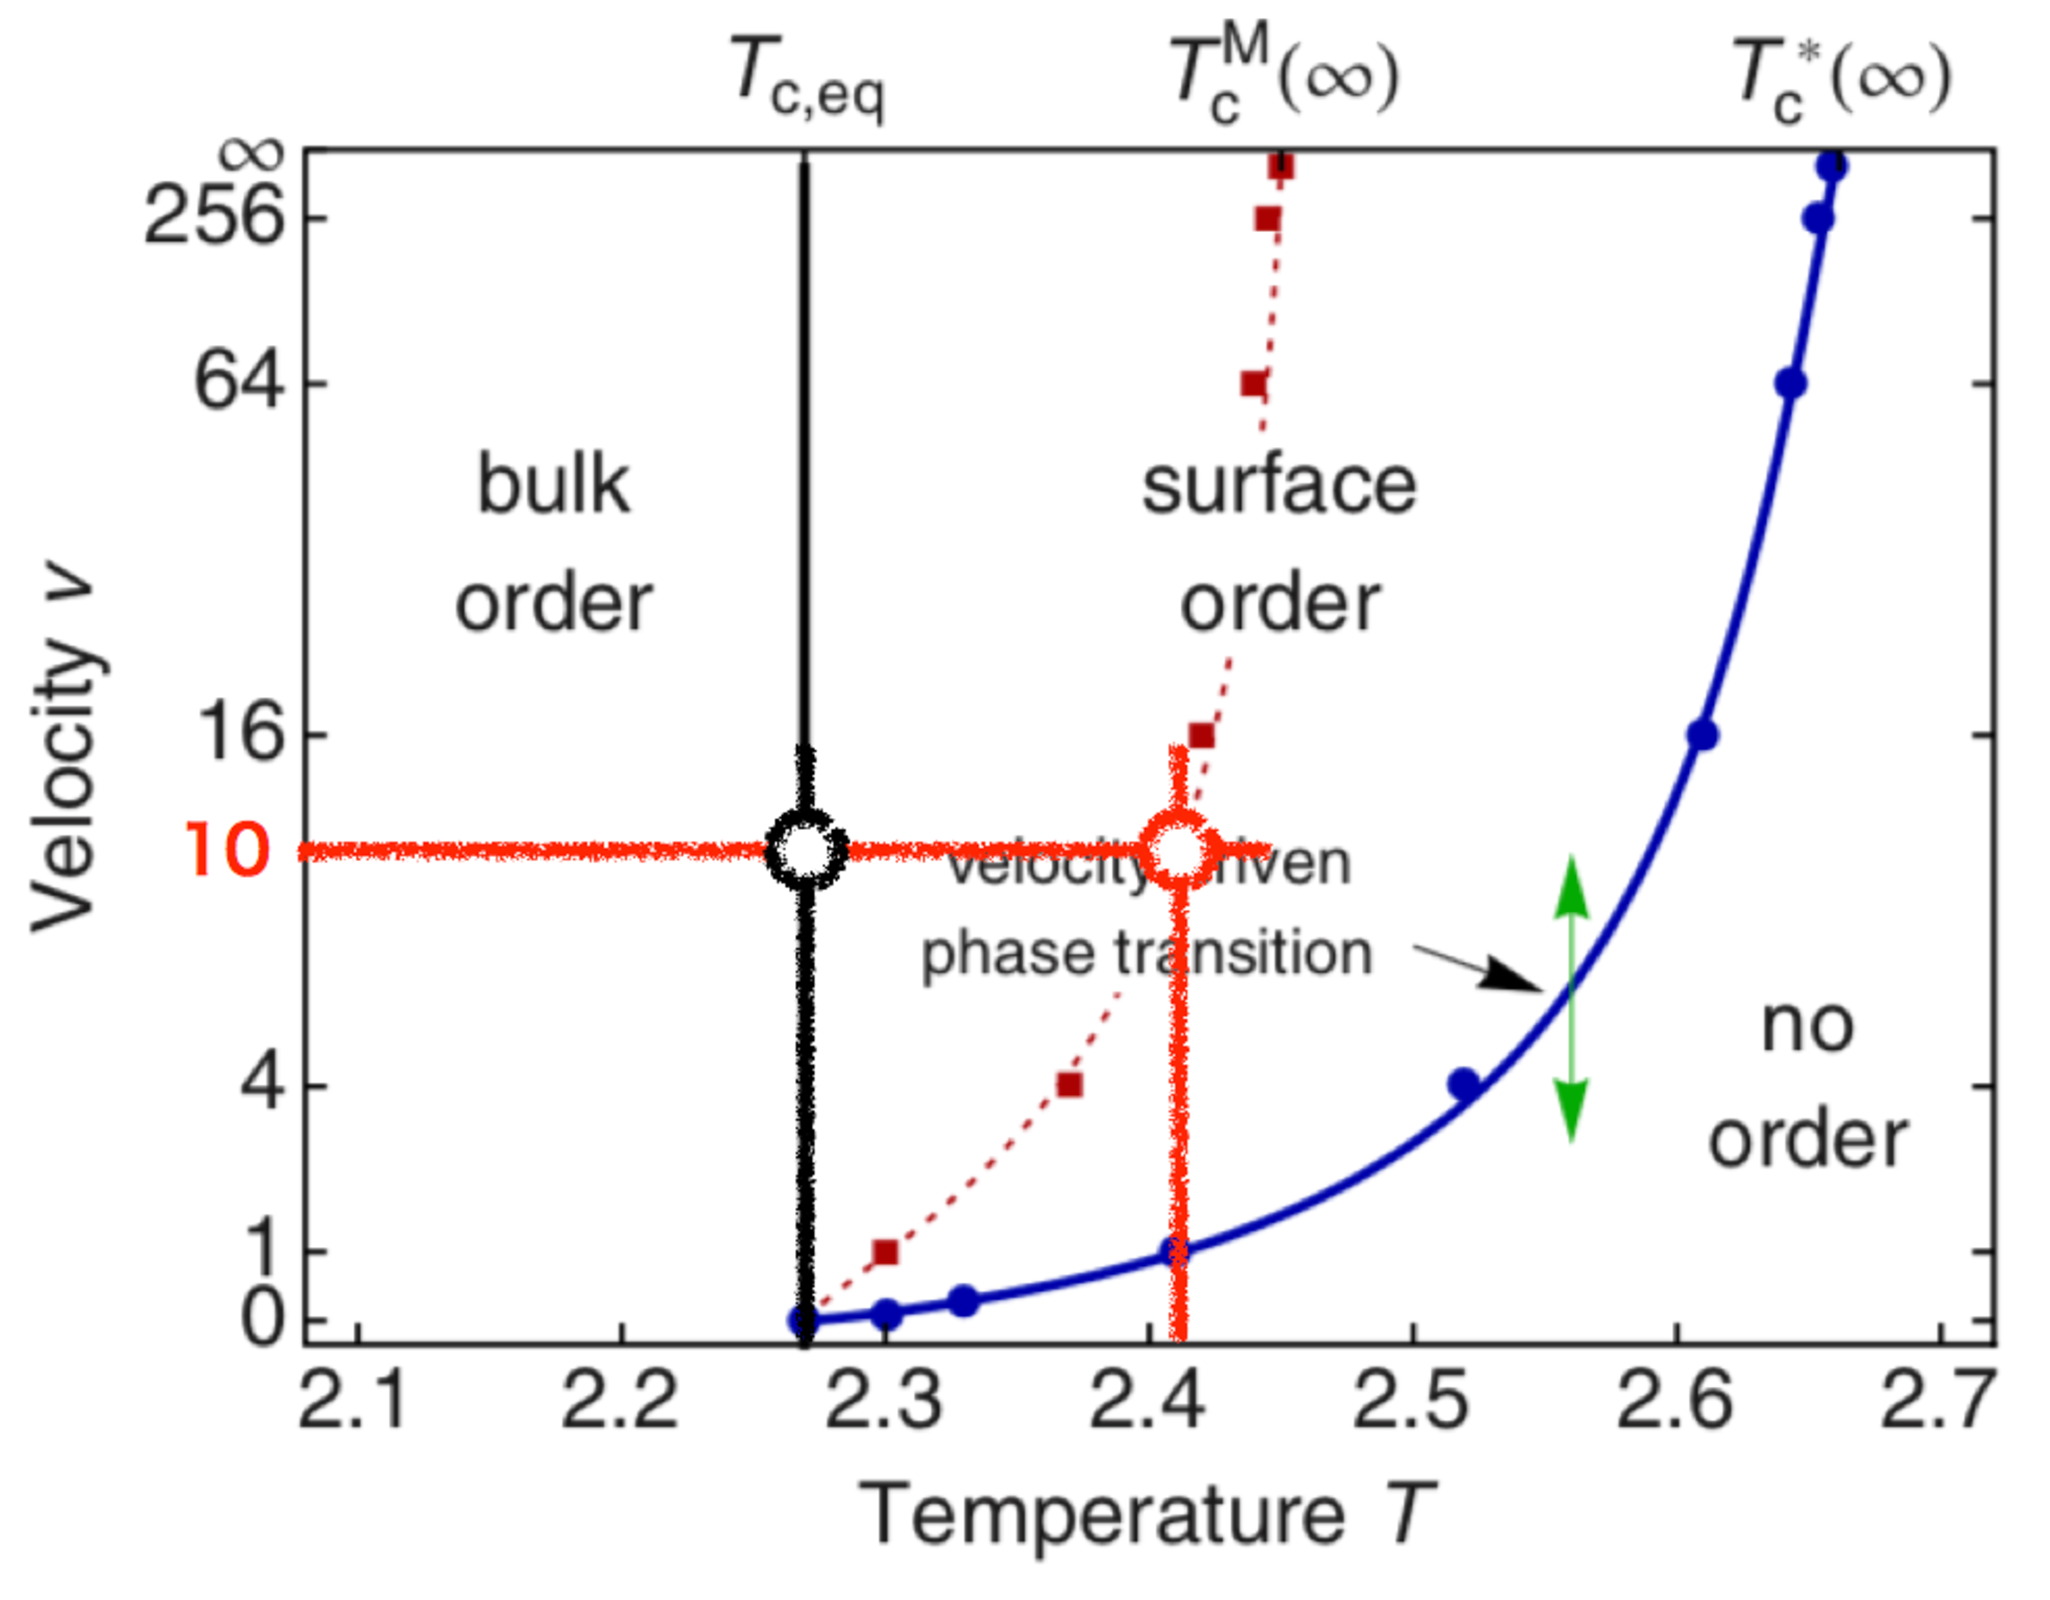
\includegraphics[width=0.5\linewidth]{NEPTIsing_.pdf}
	\caption{The non-equilibrium critical temperature $T^{\rm M}_{\rm c}(v)\simeq 2.40$ (the vertical red line) with the velocity $v\simeq 10$ and the equilibrium critical temperature $T_{\rm c, eq}\simeq 2.27$ (the vertical black line) in the phase diagram of the two-dimensional non-equilibrium Ising model obtained in Ref.~\cite{Hucht2009b}\protect\footnotemark.}
	\label{fig:NEPTinIsing_}
\end{figure}

\footnotetext{Reprinted Fig.~15 with permission from \fullcite{Hucht2009b}. Copyright (2018) by the American Physical Society.}

We also consider the reason why not only the heat capacity $c(L_{z}, T)$ but also the temperature derivative of the frictional force density $\partial f(L_{z}, T)/\partial T$ shows the divergent behavior. The frictional force density $f(L_{z}, T)$ is estimated by the difference between the expectation value of the energy before and after the sliding. It is therefore plausible that both expectation values have a singularity near $k_{\rm B}T/J=2.40$, and these singularities do not cancel with each other.

\section{Checking the Convergence in the Limit $L_{x}\to\infty$}
\label{sec:convcheck}

We now demonstrate that the following two observables converge in the infinite-size limit $L_{x}\to\infty$:

\begin{align}
f(L_{z}, T):=&\lim_{L_{x}\to\infty}\frac{F(L_{x}, L_{z}, T)}{L_{x}},\\
\epsilon(L_{z}, T):=&\lim_{L_{x}\to\infty}\frac{E_{b}(L_{x}. L_{z}, T)}{L_{x}L_{z}}.
\end{align}
We use the aspect ratios of $L_{x}=30\times L_{z}, 40\times L_{z}, 50\times L_{z}$ with $L_{z}$ fixed in order to check the convergence in the limit $L_{x}/L_{z}\to\infty$. Figures~\ref{fig:ffdcheck1}, \ref{fig:ffdcheck2}, \ref{fig:ebcheck1} and \ref{fig:ebcheck2} respectively show the temperature dependence of the frictional force density and the energy density under each set of boundary conditions for each size of $L_{z} = 4, 8, 16, 32, 64$. We see the quantities $F(L_{x}, L_{z}, T)/L_{x}$ and $E(L_{x}, L_{z}, T)/L_{x}$ for each set of boundary conditions have little dependence on $L_{x}$ for sufficiently large size of $L_{x}$ with each size of $L_{z}$.

\begin{figure}[htbp]
	\centering
	\subcaptionbox{\label{fig:ffdcheckfor004}}[0.80\linewidth]{\includegraphics[width=0.55\linewidth]{../../NumCalc/ClassicalSpinMC/FricDensP_Lz004.eps}}
	
	\subcaptionbox{\label{fig:ffdcheckfor008}}[0.80\linewidth]{\includegraphics[width=0.55\linewidth]{../../NumCalc/ClassicalSpinMC/FricDensP_Lz008.eps}}
	
	\subcaptionbox{\label{fig:ffdcheckfor016}}[0.80\linewidth]{\includegraphics[width=0.55\linewidth]{../../NumCalc/ClassicalSpinMC/FricDensP_Lz016.eps}}
	
	\caption{Each panel shows $F(L_{x}, L_{z}, T)/L_{x}$ against the temperature $T$: (\subref{fig:ffdcheckfor004}) $L_{z}=4$; (\subref{fig:ffdcheckfor008}) $L_{z}=8$; (\subref{fig:ffdcheckfor016}) $L_{z}=16$.}
	\label{fig:ffdcheck1}
\end{figure}

\begin{figure}[htbp]
	\centering
	\subcaptionbox{\label{fig:ffdcheckfor032}}[0.80\linewidth]{\includegraphics[width=0.55\linewidth]{../../NumCalc/ClassicalSpinMC/FricDensP_Lz032.eps}}
	
	\subcaptionbox{\label{fig:ffdcheckfor064}}[0.80\linewidth]{\includegraphics[width=0.55\linewidth]{../../NumCalc/ClassicalSpinMC/FricDensP_Lz064.eps}}
	
	\caption{Each panel shows $F(L_{x}, L_{z}, T)/L_{x}$ against the temperature $T$: (\subref{fig:ffdcheckfor032}) $L_{z}=32$; (\subref{fig:ffdcheckfor064}) $L_{z}=64$.}
	\label{fig:ffdcheck2}
\end{figure}

\begin{figure}[htbp]
	\centering
	\subcaptionbox{\label{fig:ebcheckfor004}}[0.80\linewidth]{\includegraphics[width=0.55\linewidth]{../../NumCalc/ClassicalSpinMC/EnDens_Lz004.eps}}
	
	\subcaptionbox{\label{fig:ebcheckfor008}}[0.80\linewidth]{\includegraphics[width=0.55\linewidth]{../../NumCalc/ClassicalSpinMC/EnDens_Lz008.eps}}
	
	\subcaptionbox{\label{fig:ebcheckfor016}}[0.80\linewidth]{\includegraphics[width=0.55\linewidth]{../../NumCalc/ClassicalSpinMC/EnDens_Lz016.eps}}
	
	\caption{Each panel shows $E(L_{x}, L_{z}, T)/(L_{x}L_{z})$ against the temperature $T$: (\subref{fig:ffdcheckfor004}) $L_{z}=4$; (\subref{fig:ffdcheckfor008}) $L_{z}=8$; (\subref{fig:ffdcheckfor016}) $L_{z}=16$.}
	\label{fig:ebcheck1}
\end{figure}

\begin{figure}[htbp]
	\centering
	\subcaptionbox{\label{fig:ebcheckfor032}}[0.80\linewidth]{\includegraphics[width=0.55\linewidth]{../../NumCalc/ClassicalSpinMC/EnDens_Lz032.eps}}
	
	\subcaptionbox{\label{fig:ebcheckfor064}}[0.80\linewidth]{\includegraphics[width=0.55\linewidth]{../../NumCalc/ClassicalSpinMC/EnDens_Lz064.eps}}
	
	\caption{Each panel shows $E(L_{x}, L_{z}, T)/(L_{x}L_{z})$ against the temperature $T$: (\subref{fig:ffdcheckfor032}) $L_{z}=32$; (\subref{fig:ffdcheckfor064}) $L_{z}=64$.}
	\label{fig:ebcheck2}
\end{figure}

%\section{Time Series of Observables}\label{appsec:timeconvcheck}
%
%\renewcommand\thefigure{\thesection.\arabic{figure}}
%\renewcommand\thesubfigure{\thefigure.\arabic{subfigure}}
%
%We now show the data which we use to calculate the long time limit of power  $P(t)$, dissipation rate $D(t)$ and bulk energy $E_{\rm b}(t)$.
%
%We can estimate the non-equilibrium correlation time of these observables, and then the valid interval in each time series are determined.
%
%\subsection{Bulk Energy Densities for the Anti-parallel Boundary Condition}
%
%\subsubsection{With the Size of $L_{z}=4$, $L_{x}=40$}
%\begin{figure}[htbp]
%	\centering
%	\subcaptionbox{$k_{\rm B}T/J=5.0$}{\includegraphics[width=0.3\linewidth]{../../NumCalc/ClassicalSpinMC/dat/Lz004Lx0040Ly__Vel10/antiparallel/ed_beta.200.eps}}
%	\subcaptionbox{$k_{\rm B}T/J=4.9$}{\includegraphics[width=0.3\linewidth]{../../NumCalc/ClassicalSpinMC/dat/Lz004Lx0040Ly__Vel10/antiparallel/ed_beta.204.eps}}
%	\subcaptionbox{$k_{\rm B}T/J=4.8$}{\includegraphics[width=0.3\linewidth]{../../NumCalc/ClassicalSpinMC/dat/Lz004Lx0040Ly__Vel10/antiparallel/ed_beta.208.eps}}
%
%	\subcaptionbox{$k_{\rm B}T/J=4.7$}{\includegraphics[width=0.3\linewidth]{../../NumCalc/ClassicalSpinMC/dat/Lz004Lx0040Ly__Vel10/antiparallel/ed_beta.212.eps}}
%	\subcaptionbox{$k_{\rm B}T/J=4.6$}{\includegraphics[width=0.3\linewidth]{../../NumCalc/ClassicalSpinMC/dat/Lz004Lx0040Ly__Vel10/antiparallel/ed_beta.217.eps}}
%	\subcaptionbox{$k_{\rm B}T/J=4.5$}{\includegraphics[width=0.3\linewidth]{../../NumCalc/ClassicalSpinMC/dat/Lz004Lx0040Ly__Vel10/antiparallel/ed_beta.222.eps}}
%
%	\subcaptionbox{$k_{\rm B}T/J=4.4$}{\includegraphics[width=0.3\linewidth]{../../NumCalc/ClassicalSpinMC/dat/Lz004Lx0040Ly__Vel10/antiparallel/ed_beta.227.eps}}
%	\subcaptionbox{$k_{\rm B}T/J=4.3$}{\includegraphics[width=0.3\linewidth]{../../NumCalc/ClassicalSpinMC/dat/Lz004Lx0040Ly__Vel10/antiparallel/ed_beta.232.eps}}
%	\subcaptionbox{$k_{\rm B}T/J=4.2$}{\includegraphics[width=0.3\linewidth]{../../NumCalc/ClassicalSpinMC/dat/Lz004Lx0040Ly__Vel10/antiparallel/ed_beta.238.eps}}
%
%	\subcaptionbox{$k_{\rm B}T/J=4.1$}{\includegraphics[width=0.3\linewidth]{../../NumCalc/ClassicalSpinMC/dat/Lz004Lx0040Ly__Vel10/antiparallel/ed_beta.243.eps}}
%	\subcaptionbox{$k_{\rm B}T/J=4.0$}{\includegraphics[width=0.3\linewidth]{../../NumCalc/ClassicalSpinMC/dat/Lz004Lx0040Ly__Vel10/antiparallel/ed_beta.250.eps}}
%	\subcaptionbox{$k_{\rm B}T/J=3.9$}{\includegraphics[width=0.3\linewidth]{../../NumCalc/ClassicalSpinMC/dat/Lz004Lx0040Ly__Vel10/antiparallel/ed_beta.256.eps}}
%
%	\subcaptionbox{$k_{\rm B}T/J=3.8$}{\includegraphics[width=0.3\linewidth]{../../NumCalc/ClassicalSpinMC/dat/Lz004Lx0040Ly__Vel10/antiparallel/ed_beta.263.eps}}
%	\subcaptionbox{$k_{\rm B}T/J=3.7$}{\includegraphics[width=0.3\linewidth]{../../NumCalc/ClassicalSpinMC/dat/Lz004Lx0040Ly__Vel10/antiparallel/ed_beta.270.eps}}
%	\subcaptionbox{$k_{\rm B}T/J=3.6$}{\includegraphics[width=0.3\linewidth]{../../NumCalc/ClassicalSpinMC/dat/Lz004Lx0040Ly__Vel10/antiparallel/ed_beta.277.eps}}
%	
%	\caption{Each data shows $\epsilon_{\rm b}(L_{x}, L_{z}, T)/(L_{x}L_{z})$ versus $t$.}
%\end{figure}
%
%\begin{figure}[htbp]
%	\centering
%	\subcaptionbox{$k_{\rm B}T/J=3.5$}{\includegraphics[width=0.3\linewidth]{../../NumCalc/ClassicalSpinMC/dat/Lz004Lx0040Ly__Vel10/antiparallel/ed_beta.285.eps}}
%	\subcaptionbox{$k_{\rm B}T/J=3.4$}{\includegraphics[width=0.3\linewidth]{../../NumCalc/ClassicalSpinMC/dat/Lz004Lx0040Ly__Vel10/antiparallel/ed_beta.294.eps}}
%	\subcaptionbox{$k_{\rm B}T/J=3.3$}{\includegraphics[width=0.3\linewidth]{../../NumCalc/ClassicalSpinMC/dat/Lz004Lx0040Ly__Vel10/antiparallel/ed_beta.303.eps}}
%
%	\subcaptionbox{$k_{\rm B}T/J=3.2$}{\includegraphics[width=0.3\linewidth]{../../NumCalc/ClassicalSpinMC/dat/Lz004Lx0040Ly__Vel10/antiparallel/ed_beta.312.eps}}
%	\subcaptionbox{$k_{\rm B}T/J=3.1$}{\includegraphics[width=0.3\linewidth]{../../NumCalc/ClassicalSpinMC/dat/Lz004Lx0040Ly__Vel10/antiparallel/ed_beta.322.eps}}
%	\subcaptionbox{$k_{\rm B}T/J=3.0$}{\includegraphics[width=0.3\linewidth]{../../NumCalc/ClassicalSpinMC/dat/Lz004Lx0040Ly__Vel10/antiparallel/ed_beta.333.eps}}
%
%	\subcaptionbox{$k_{\rm B}T/J=2.9$}{\includegraphics[width=0.3\linewidth]{../../NumCalc/ClassicalSpinMC/dat/Lz004Lx0040Ly__Vel10/antiparallel/ed_beta.344.eps}}
%	\subcaptionbox{$k_{\rm B}T/J=2.8$}{\includegraphics[width=0.3\linewidth]{../../NumCalc/ClassicalSpinMC/dat/Lz004Lx0040Ly__Vel10/antiparallel/ed_beta.357.eps}}
%	\subcaptionbox{$k_{\rm B}T/J=2.7$}{\includegraphics[width=0.3\linewidth]{../../NumCalc/ClassicalSpinMC/dat/Lz004Lx0040Ly__Vel10/antiparallel/ed_beta.370.eps}}
%
%	\subcaptionbox{$k_{\rm B}T/J=2.6$}{\includegraphics[width=0.3\linewidth]{../../NumCalc/ClassicalSpinMC/dat/Lz004Lx0040Ly__Vel10/antiparallel/ed_beta.384.eps}}
%	\subcaptionbox{$k_{\rm B}T/J=2.50$}{\includegraphics[width=0.3\linewidth]{../../NumCalc/ClassicalSpinMC/dat/Lz004Lx0040Ly__Vel10/antiparallel/ed_beta.400.eps}}
%	\subcaptionbox{$k_{\rm B}T/J=2.48$}{\includegraphics[width=0.3\linewidth]{../../NumCalc/ClassicalSpinMC/dat/Lz004Lx0040Ly__Vel10/antiparallel/ed_beta.403.eps}}
%
%	\subcaptionbox{$k_{\rm B}T/J=2.46$}{\includegraphics[width=0.3\linewidth]{../../NumCalc/ClassicalSpinMC/dat/Lz004Lx0040Ly__Vel10/antiparallel/ed_beta.406.eps}}
%	\subcaptionbox{$k_{\rm B}T/J=2.44$}{\includegraphics[width=0.3\linewidth]{../../NumCalc/ClassicalSpinMC/dat/Lz004Lx0040Ly__Vel10/antiparallel/ed_beta.409.eps}}
%	\subcaptionbox{$k_{\rm B}T/J=2.42$}{\includegraphics[width=0.3\linewidth]{../../NumCalc/ClassicalSpinMC/dat/Lz004Lx0040Ly__Vel10/antiparallel/ed_beta.413.eps}}
%	
%	\caption{Each data shows $\epsilon_{\rm b}(L_{x}, L_{z}, T)/(L_{x}L_{z})$ versus $t$.}
%\end{figure}
%
%\begin{figure}[htbp]
%	\centering
%	\subcaptionbox{$k_{\rm B}T/J=2.40$}{\includegraphics[width=0.3\linewidth]{../../NumCalc/ClassicalSpinMC/dat/Lz004Lx0040Ly__Vel10/antiparallel/ed_beta.416.eps}}
%	\subcaptionbox{$k_{\rm B}T/J=2.38$}{\includegraphics[width=0.3\linewidth]{../../NumCalc/ClassicalSpinMC/dat/Lz004Lx0040Ly__Vel10/antiparallel/ed_beta.420.eps}}
%	\subcaptionbox{$k_{\rm B}T/J=2.36$}{\includegraphics[width=0.3\linewidth]{../../NumCalc/ClassicalSpinMC/dat/Lz004Lx0040Ly__Vel10/antiparallel/ed_beta.423.eps}}
%
%	\subcaptionbox{$k_{\rm B}T/J=2.34$}{\includegraphics[width=0.3\linewidth]{../../NumCalc/ClassicalSpinMC/dat/Lz004Lx0040Ly__Vel10/antiparallel/ed_beta.427.eps}}
%	\subcaptionbox{$k_{\rm B}T/J=2.32$}{\includegraphics[width=0.3\linewidth]{../../NumCalc/ClassicalSpinMC/dat/Lz004Lx0040Ly__Vel10/antiparallel/ed_beta.431.eps}}
%	\subcaptionbox{$k_{\rm B}T/J=2.30$}{\includegraphics[width=0.3\linewidth]{../../NumCalc/ClassicalSpinMC/dat/Lz004Lx0040Ly__Vel10/antiparallel/ed_beta.434.eps}}
%
%	\subcaptionbox{$k_{\rm B}T/J=2.26$}{\includegraphics[width=0.3\linewidth]{../../NumCalc/ClassicalSpinMC/dat/Lz004Lx0040Ly__Vel10/antiparallel/ed_beta.442.eps}}
%	\subcaptionbox{$k_{\rm B}T/J=2.24$}{\includegraphics[width=0.3\linewidth]{../../NumCalc/ClassicalSpinMC/dat/Lz004Lx0040Ly__Vel10/antiparallel/ed_beta.446.eps}}
%	\subcaptionbox{$k_{\rm B}T/J=2.22$}{\includegraphics[width=0.3\linewidth]{../../NumCalc/ClassicalSpinMC/dat/Lz004Lx0040Ly__Vel10/antiparallel/ed_beta.450.eps}}
%
%	\subcaptionbox{$k_{\rm B}T/J=2.20$}{\includegraphics[width=0.3\linewidth]{../../NumCalc/ClassicalSpinMC/dat/Lz004Lx0040Ly__Vel10/antiparallel/ed_beta.454.eps}}
%	\subcaptionbox{$k_{\rm B}T/J=2.18$}{\includegraphics[width=0.3\linewidth]{../../NumCalc/ClassicalSpinMC/dat/Lz004Lx0040Ly__Vel10/antiparallel/ed_beta.458.eps}}
%	\subcaptionbox{$k_{\rm B}T/J=2.16$}{\includegraphics[width=0.3\linewidth]{../../NumCalc/ClassicalSpinMC/dat/Lz004Lx0040Ly__Vel10/antiparallel/ed_beta.462.eps}}
%
%	\subcaptionbox{$k_{\rm B}T/J=2.14$}{\includegraphics[width=0.3\linewidth]{../../NumCalc/ClassicalSpinMC/dat/Lz004Lx0040Ly__Vel10/antiparallel/ed_beta.467.eps}}
%	\subcaptionbox{$k_{\rm B}T/J=2.12$}{\includegraphics[width=0.3\linewidth]{../../NumCalc/ClassicalSpinMC/dat/Lz004Lx0040Ly__Vel10/antiparallel/ed_beta.471.eps}}
%	\subcaptionbox{$k_{\rm B}T/J=2.10$}{\includegraphics[width=0.3\linewidth]{../../NumCalc/ClassicalSpinMC/dat/Lz004Lx0040Ly__Vel10/antiparallel/ed_beta.476.eps}}
%	\caption{Each data shows $\epsilon_{\rm b}(L_{x}, L_{z}, T)/(L_{x}L_{z})$ versus $t$.}
%\end{figure}
%
%\begin{figure}[htbp]
%	\centering
%	\subcaptionbox{$k_{\rm B}T/J=2.08$}{\includegraphics[width=0.3\linewidth]{../../NumCalc/ClassicalSpinMC/dat/Lz004Lx0040Ly__Vel10/antiparallel/ed_beta.480.eps}}
%	\subcaptionbox{$k_{\rm B}T/J=2.06$}{\includegraphics[width=0.3\linewidth]{../../NumCalc/ClassicalSpinMC/dat/Lz004Lx0040Ly__Vel10/antiparallel/ed_beta.485.eps}}
%	\subcaptionbox{$k_{\rm B}T/J=2.04$}{\includegraphics[width=0.3\linewidth]{../../NumCalc/ClassicalSpinMC/dat/Lz004Lx0040Ly__Vel10/antiparallel/ed_beta.490.eps}}
%
%	\subcaptionbox{$k_{\rm B}T/J=2.02$}{\includegraphics[width=0.3\linewidth]{../../NumCalc/ClassicalSpinMC/dat/Lz004Lx0040Ly__Vel10/antiparallel/ed_beta.495.eps}}
%	\subcaptionbox{$k_{\rm B}T/J=1.9$}{\includegraphics[width=0.3\linewidth]{../../NumCalc/ClassicalSpinMC/dat/Lz004Lx0040Ly__Vel10/antiparallel/ed_beta.526.eps}}
%	\subcaptionbox{$k_{\rm B}T/J=1.8$}{\includegraphics[width=0.3\linewidth]{../../NumCalc/ClassicalSpinMC/dat/Lz004Lx0040Ly__Vel10/antiparallel/ed_beta.555.eps}}
%
%	\subcaptionbox{$k_{\rm B}T/J=1.7$}{\includegraphics[width=0.3\linewidth]{../../NumCalc/ClassicalSpinMC/dat/Lz004Lx0040Ly__Vel10/antiparallel/ed_beta.588.eps}}
%	\subcaptionbox{$k_{\rm B}T/J=1.6$}{\includegraphics[width=0.3\linewidth]{../../NumCalc/ClassicalSpinMC/dat/Lz004Lx0040Ly__Vel10/antiparallel/ed_beta.625.eps}}
%	\subcaptionbox{$k_{\rm B}T/J=1.5$}{\includegraphics[width=0.3\linewidth]{../../NumCalc/ClassicalSpinMC/dat/Lz004Lx0040Ly__Vel10/antiparallel/ed_beta.666.eps}}
%
%	\subcaptionbox{$k_{\rm B}T/J=1.4$}{\includegraphics[width=0.3\linewidth]{../../NumCalc/ClassicalSpinMC/dat/Lz004Lx0040Ly__Vel10/antiparallel/ed_beta.714.eps}}
%	\subcaptionbox{$k_{\rm B}T/J=1.3$}{\includegraphics[width=0.3\linewidth]{../../NumCalc/ClassicalSpinMC/dat/Lz004Lx0040Ly__Vel10/antiparallel/ed_beta.769.eps}}
%	\subcaptionbox{$k_{\rm B}T/J=1.2$}{\includegraphics[width=0.3\linewidth]{../../NumCalc/ClassicalSpinMC/dat/Lz004Lx0040Ly__Vel10/antiparallel/ed_beta.833.eps}}
%
%	\subcaptionbox{$k_{\rm B}T/J=1.1$}{\includegraphics[width=0.3\linewidth]{../../NumCalc/ClassicalSpinMC/dat/Lz004Lx0040Ly__Vel10/antiparallel/ed_beta.909.eps}}
%	\subcaptionbox{$k_{\rm B}T/J=1.0$}{\includegraphics[width=0.3\linewidth]{../../NumCalc/ClassicalSpinMC/dat/Lz004Lx0040Ly__Vel10/antiparallel/ed_beta1.000.eps}}
%	\subcaptionbox{$k_{\rm B}T/J=0.9$}{\includegraphics[width=0.3\linewidth]{../../NumCalc/ClassicalSpinMC/dat/Lz004Lx0040Ly__Vel10/antiparallel/ed_beta1.111.eps}}
%	\caption{Each data shows $\epsilon_{\rm b}(L_{x}, L_{z}, T)/(L_{x}L_{z})$ versus $t$.}
%\end{figure}
%
%\begin{figure}[htbp]
%	\centering
%	\subcaptionbox{$k_{\rm B}T/J=0.8$}{\includegraphics[width=0.3\linewidth]{../../NumCalc/ClassicalSpinMC/dat/Lz004Lx0040Ly__Vel10/antiparallel/ed_beta1.250.eps}}
%	\subcaptionbox{$k_{\rm B}T/J=0.7$}{\includegraphics[width=0.3\linewidth]{../../NumCalc/ClassicalSpinMC/dat/Lz004Lx0040Ly__Vel10/antiparallel/ed_beta1.428.eps}}
%	\subcaptionbox{$k_{\rm B}T/J=0.6$}{\includegraphics[width=0.3\linewidth]{../../NumCalc/ClassicalSpinMC/dat/Lz004Lx0040Ly__Vel10/antiparallel/ed_beta1.666.eps}}
%
%	\subcaptionbox{$k_{\rm B}T/J=0.5$}{\includegraphics[width=0.3\linewidth]{../../NumCalc/ClassicalSpinMC/dat/Lz004Lx0040Ly__Vel10/antiparallel/ed_beta2.000.eps}}
%	\subcaptionbox{$k_{\rm B}T/J=0.4$}{\includegraphics[width=0.3\linewidth]{../../NumCalc/ClassicalSpinMC/dat/Lz004Lx0040Ly__Vel10/antiparallel/ed_beta2.500.eps}}
%	\subcaptionbox{$k_{\rm B}T/J=0.3$}{\includegraphics[width=0.3\linewidth]{../../NumCalc/ClassicalSpinMC/dat/Lz004Lx0040Ly__Vel10/antiparallel/ed_beta3.333.eps}}
%
%	\subcaptionbox{$k_{\rm B}T/J=0.2$}{\includegraphics[width=0.3\linewidth]{../../NumCalc/ClassicalSpinMC/dat/Lz004Lx0040Ly__Vel10/antiparallel/ed_beta5.000.eps}}
%	\subcaptionbox{$k_{\rm B}T/J=0.1$}{\includegraphics[width=0.3\linewidth]{../../NumCalc/ClassicalSpinMC/dat/Lz004Lx0040Ly__Vel10/antiparallel/ed_beta10.000.eps}}
%	\caption{Each data shows $\epsilon_{\rm b}(L_{x}, L_{z}, T)/(L_{x}L_{z})$ versus $t$.}
%\end{figure}
%
%\subsubsection{With the Size of $L_{z}=4$, $L_{x}=80$}
%
%\subsubsection{With the Size of $L_{z}=4$, $L_{x}=120$}
%
%\subsubsection{With the Size of $L_{z}=4$, $L_{x}=160$}
%
%\subsubsection{With the Size of $L_{z}=4$, $L_{x}=300$}
%
%\subsection{Bulk Energy Densities for the Parallel Boundary Condition}

% !TeX root = Body.tex
\chapter{Summary and Discussion}\label{chap:Summary}

We investigated the effects of boundary conditions on the physical quantities by non-equilibrium Monte Carlo simulations. To summarize the present results, we found that the fixed boundary conditions have an effect on the magnetic friction as an effective field; the anti-parallel and the parallel boundary conditions have disordering and ordering effects, respectively. These effects emerge at the sliding boundary when the system behaves as a one-dimensional system, but vanish in the two-dimensional limit. The crossover between the one dimension and the two dimensions occurs below the size $L_{z}=64$ in the limit $L_{x}\to\infty$. 

In other words, if we set the size $L_{z}$ much less (greater) than the correlation length $\xi_{z}(\beta)$ the system behaves as the one-dimensional (two-dimensional). The two sets of boundary conditions, in particular, have maximum effects on the magnetic friction when the temperature of the system is near the boundary critical temperature and the system is sufficiently thin.

Thereby we propose to manipulate the magnetic friction by switching the one boundary condition into the other near the boundary criticality. We can thus sharply increase and decrease the magnetic friction. 

In order to be more precise, we should calculate the correlation length along the $z$ direction $\xi_{z}(\beta)$. Its definition may be different from that of the equilibrium case because the homogeneity along the $z$ direction is destroyed by the constant sliding motion. A good definition of $\xi_{z}(\beta)$ could give the dimensional crossover point by the following way.

%For the temperature near the critical point, in general, the correlation length behaves as $\xi \simeq t^{-\nu}$, where $t$ and $\nu$ denote the reduced temperature $(T-T_{c})/T_{c}$ and the critical exponent, respectively. The correlation function is written by $\langle \sigma_{i}\sigma_{j}\rangle \simeq \mathrm{e}^{-|i-j|/\xi}$. This leads the following relation:
%\begin{align}
%\langle \sigma_{i}\sigma_{j}\rangle &\simeq \exp\left[-|i-j|t^{\nu}\right],\\
%\Longleftrightarrow \nu &\simeq \log\left[-\frac{\log \langle \sigma_{i}\sigma_{j}\rangle}{|i-j|}\right]/\log t\label{rel:effcritexp}.
%\end{align}
%
%The right-hand side of \eqref{rel:effcritexp} is expected to be equal to its universality class in each symmetries and dimensions. Thus we can able to discover the crossover phenomena by a value of r.h.s of \eqref{rel:effcritexp} which does not belongs to any universality class.
For further analysis, it is worthwhile to determine critical exponents of the non-equilibrium phase transition. We can determine the critical exponent $\alpha$ of the bulk heat capacity $c(T)$ in Fig.~\ref{fig:dEnDens_Allsize} as well as the boundary heat capacity $c_{\rm b}(T)$ by further calculations. Similarly we have critical exponents $\nu$, $\beta$ and $\gamma$ of the correlation length along $x$-direction $\xi_{x}$, the boundary magnetization $m_{b}$ and the boundary susceptibility $\chi_{b,\rm abs}$, respectively, by the methods in Ref.~\cite{Hucht2009b}, which enables us to discuss a crossover from the one-dimension to the two-dimension by the varying size $L_{z}$.

According to Ref.~\cite{Hucht2009b}, the scaling relation $2-\alpha=2\beta+\gamma=d_{\rm b}\nu$ where $d_{\rm b}$ denote the boundary dimension of the system for each bulk dimension and geometry. We can expect that the set of critical exponents exhibits a continuous change with holding the scaling relation.

The discussions on the experimental method of manipulating the magnetic friction and determination of the crossover point with more accuracy are applicable to any lattice system which can be simulated by our way. For more practical purposes, it is more important to study three-dimensional systems with two-dimensional surfaces. We intend to seek the way of manipulating the friction in three dimensional systems for future work.
%
%For future works, we are going to investigate the following:
%\begin{itemize}
%\item the divergence of derivatives of the \textit{boundary} heat capacity in the limit of $L_{z}\to\infty$;
%\item the behavior of the correlation length itself;
%\item the dimensional crossover from the viewpoint of critical exponents.
%\end{itemize}
%We also intend to see whether dimensional crossovers occur in models with other spatial dimensions or continuous symmetries.
\appendix
% !TeX root = Body.tex

\chapter{Proof of the existence of NESS}
\label{chap:ProofEx}

\section{Stochastic Matrices for Ordinary Monte Carlo Simulations}

Monte Carlo simulation extracts the relevant subspace from the true state space instead of calculating the partition function of the system, using the stochastic process. The subspace depends on the temperature, where we can approximately calculate observables.

We now consider a matrix form of the stochastic process. For example, one-dimensional Ising chain with $N$-spins has $2^{N}$ states, thus we can label each state by $i=1,2,\dots,2^{N}$. Under the assumption of stochastic time evolution, we can also define the probability $p_{i}(t)$ that the system is in the $i$-th state at a time $t$.

Furthermore, we denote the conditional probability $\tilde{p}_{ij}(t)$ that the system is in the $j$-th state at a time $t$ and in the $i$-th state at the next time $t+1$, we can define the transition probability $M_{ij}$ from the $i$-th state to the $j$-th state by
\begin{align}
\tilde{p}_{ij}(t + 1) = M_{ij} p_{j}(t)\quad\text{for $1\leq i,j\leq 2^{N}$}.
\end{align}
From the property of $p_{i}(t)$ as the probability, it should hold that $\sum_{i=1}^{2^{N}}p_{i}(t)=1$ and $p_{i}(t) \ge 0$ ($i=1,2,\dots,2^{N}$). In addition, summation $\tilde{p}_{ij}(t)$ over all previous states $j=1,2,\dots,2^{N}$ is nothing but $p_{i}(t+1)$:
\begin{align}
p_{i}(t+1) = \sum_{j=1}^{2^{N}}\tilde{p}_{ij}(t + 1) = \sum_{j=1}^{2^{N}}M_{ij}p_{j}(t)\quad\text{for $1\leq i\leq 2^{N}$}.
\end{align}
Therefore the system can be described by the stochastic time evolution of the probability vector $\bm{p}(t):={}^{\rm t}\left(p_{1}(t),p_{2}(t),\dots,p_{2^{N}}(t)\right)$ by the stochastic matrix $\hat{M}:=\left(M_{ij}\right)$:
\begin{align}
\bm{p}(t + 1) = \hat{M}\bm{p}(t).
\end{align}
The normalization property of $\{p_{i}(t)\}$ is expressed as the $L^{1}$-norm property of $\bm{p}(t)$:
\begin{align}
\|\bm{p}(t)\|_{1} = 1,
\end{align}
where the $L^{1}$-norm is defined for any vector $\bm{x}={}^{\rm t}\left(x_{1},x_{2},\dots,x_{2^{N}}\right)$ by $\|\bm{x}\|:=\sum_{i=1}^{2^{N}}x_{i}$. And it leads that
\begin{align}
&\sum_{i=1}^{2^{N}}p_{i}(t + 1) = \sum_{i=1}^{2^{N}}\sum_{j=1}^{2^{N}}M_{ij}p_{j}(t) = \sum_{j=1}^{2^{N}} \left(\sum_{i=1}^{2^{N}}M_{ij}\right)p_{j}(t),\\
\overset{\|\bm{p}(\bullet)\|_{1} = 1.}{\Longleftrightarrow} &\sum_{i=1}^{2^{N}}M_{ij} = 1\quad\text{for $1\leq i\leq 2^{N}$}\label{con:stochmat1}.
\end{align}
In addition, we impose the non-negative condition on $M_{ij}$ as the transition probability:
\begin{align}
M_{ij}\ge 0\quad\text{for $1\leq i,j\leq 2^{N}$}\label{con:stochmat2}.
\end{align}
Any matrix with conditions \eqref{con:stochmat1} and \eqref{con:stochmat2} is called \textit{stochastic matrix} and shows following interesting properties:
\begin{itemize}
	\item All absolute values of eigenvalue are less than or equal to $1$.
	\item For any eigenvector $\bm{x}={}^{\rm t}\{x_{1},x_{2},\dots,x_{2^{N}}\}$ which does \textit{not} belong to 1, it holds that
	\begin{align}
		\sum_{i=1}^{2^{N}}x_{j}=0.
	\end{align}
\end{itemize}
Furthermore, if we use the Metropolis probability $p_{\rm M}(t)$ the stochastic matrix $\hat{M}$ which corresponds to a Monte Carlo step satisfies following property so called \textit{strong connectivity}:
\begin{align}
content...
\end{align}

\section{Stochastic Matrices for Non-Equilbrium Monte Carlo Simulations}

\section{Calculation Non-Equilbrium Observables by the Stochastic Matrices}
%% !TeX root = Body.tex

\chapter{Simulation Algorithms}

\begin{algorithm}                      
	\caption{Single Flip Algorithm for a Monte Carlo Time (Equilibrium)}         
	\label{alg:SFAEMC}                          
	\begin{algorithmic}                  
	\FOR{$i_{\rm step} = 1, \dots, N_{\rm size}$}
	\STATE randomly chose a spin
	\STATE flip by the probability $\min\{1, \mathrm{e}^{\beta \Delta E}\}$
	\ENDFOR
	\STATE measurement
	\end{algorithmic}
\end{algorithm}

\begin{algorithm}                      
	\caption{Single Flip Algorithm for a Monte Carlo Time (Non-equilibrium)}         
	\label{alg:SFANEMC}                          
	\begin{algorithmic} 
		\STATE $\text{pump} = 0$  
		\STATE $\text{diss} = 0$                     
		\FOR {$i_{\rm v} = 1, \dots, v$}
			\STATE $\text{prev}\Leftarrow \text{energy on the slip plane}$
			\STATE sliding
			\STATE $\text{next}\Leftarrow \text{energy on the slip plane}$
			\STATE $\text{pump} = \text{pump} + (\text{next} - \text{prev})$
			\\
			\STATE $\text{prev}\Leftarrow \text{energy on the entire system}$
			\FOR{$i_{\rm step} = 1, \dots, N_{\rm size}/v$}
				\STATE flip by the probability $\min\{1, \mathrm{e}^{\beta \Delta E}\}$
			\ENDFOR
			\STATE $\text{next}\Leftarrow \text{energy on the entire system}$
			\STATE $\text{diss} = \text{diss} + (\text{next} - \text{prev})$
		\ENDFOR
		\STATE{measurement}
	\end{algorithmic}
\end{algorithm}
%% !TeX root = Body.tex

\chapter{Results of Simulations in More Detail}

\section{Checking the Convergence in the Limit $L_{x}\to\infty$}
\label{appsec:convcheck}

We now demonstrate that following two observables are converging at corresponding numerical large size limits.

\begin{align}
	f(L_{z}, T):=&\lim_{L_{x}\to\infty}\frac{F(L_{x}, L_{z}, T)}{L_{x}}\\
	\epsilon_{\rm b}(L_{z}, T):=&\lim_{L_{x}\to\infty}\frac{E_{b}(L_{x}, L_{z}, T)}{L_{x}L_{z}}
\end{align}

Both of them have no dependence on $L_{x}$ and also do not diverge in the limit of $L_{z}$. Thus we can analyze these qualitative and pure dependence on $L_{z}$ and $T$. We use the aspect of $L_{x}=10L_{z}, 20L_{z}, \dots, 50L_{z}$ for checking the convergence in the limit $L_{x}/L_{z} \to \infty$ with fixed $L_{z}$.

\subsection{Dependence of $F(L_{x}, L_{z}, T)/L_{x}$ on $L_{x}$ for each $L_{z}$}

\begin{figure}[htbp]
	\centering
	\subcaptionbox{$L_{z}=4$\label{fig:ffdcheckfor004}}{\includegraphics[width=0.4\linewidth]{../../NumCalc/ClassicalSpinMC/FricDensP_Lz004.eps}}
	\subcaptionbox{$L_{z}=6$\label{fig:ffdcheckfor006}}{\includegraphics[width=0.4\linewidth]{../../NumCalc/ClassicalSpinMC/FricDensP_Lz006.eps}}
	
	\subcaptionbox{$L_{z}=8$\label{fig:ffdcheckfor008}}{\includegraphics[width=0.4\linewidth]{../../NumCalc/ClassicalSpinMC/FricDensP_Lz008.eps}}
	\subcaptionbox{$L_{z}=10$\label{fig:ffdcheckfor010}}{\includegraphics[width=0.4\linewidth]{../../NumCalc/ClassicalSpinMC/FricDensP_Lz010.eps}}
	
	\subcaptionbox{$L_{z}=12$\label{fig:ffdcheckfor012}}{\includegraphics[width=0.4\linewidth]{../../NumCalc/ClassicalSpinMC/FricDensP_Lz012.eps}}
	\subcaptionbox{$L_{z}=14$\label{fig:ffdcheckfor014}}{\includegraphics[width=0.4\linewidth]{../../NumCalc/ClassicalSpinMC/FricDensP_Lz014.eps}}
	
	\subcaptionbox{$L_{z}=16$\label{fig:ffdcheckfor016}}{\includegraphics[width=0.4\linewidth]{../../NumCalc/ClassicalSpinMC/FricDensP_Lz016.eps}}
	\caption{Each data shows $F(L_{x}, L_{z}, T)/L_{x}$ versus $T$.}
	\label{fig:ffdcheck}
\end{figure}

We show that the quantity $F(L_{x}, L_{z}, T)/L_{x}$ has no dependence on $L_{x}$ at a sufficient large $L_{x}$ for each $L_{z}$. The following graphs are the temperature dependence of the frictional force density with each of boundary conditions along the $z$-direction for each of longitudinal size $L_{z} = 4, 6, 8, 10, 12, 14, 16$ (fig.\ref{fig:ffdcheck}).

\subsection{Dependence of $E_{\rm b}(L_{x}, L_{z}, T)/(L_{x}L_{z})$ on $L_{x}$ for each $L_{z}$}

\begin{figure}[htbp]
	\centering
	\subcaptionbox{$L_{z}=4$\label{fig:ebcheckfor004}}{\includegraphics[width=0.4\linewidth]{../../NumCalc/ClassicalSpinMC/EnDens_Lz004.eps}}
	\subcaptionbox{$L_{z}=6$\label{fig:ebcheckfor006}}{\includegraphics[width=0.4\linewidth]{../../NumCalc/ClassicalSpinMC/EnDens_Lz006.eps}}
	
	\subcaptionbox{$L_{z}=8$\label{fig:ebcheckfor008}}{\includegraphics[width=0.4\linewidth]{../../NumCalc/ClassicalSpinMC/EnDens_Lz008.eps}}
	\subcaptionbox{$L_{z}=10$\label{fig:ebcheckfor010}}{\includegraphics[width=0.4\linewidth]{../../NumCalc/ClassicalSpinMC/EnDens_Lz010.eps}}
	
	\subcaptionbox{$L_{z}=12$\label{fig:ebcheckfor012}}{\includegraphics[width=0.4\linewidth]{../../NumCalc/ClassicalSpinMC/EnDens_Lz012.eps}}
	\subcaptionbox{$L_{z}=14$\label{fig:ebcheckfor014}}{\includegraphics[width=0.4\linewidth]{../../NumCalc/ClassicalSpinMC/EnDens_Lz014.eps}}
	
	\subcaptionbox{$L_{z}=16$\label{fig:ebcheckfor016}}{\includegraphics[width=0.4\linewidth]{../../NumCalc/ClassicalSpinMC/EnDens_Lz016.eps}}
	\caption{Each data shows $E(L_{x}, L_{z}, T)/(L_{x}L_{z})$ versus $T$.}
	\label{fig:ebcheck}
\end{figure}

We show that the quantity $E_{\rm b}(L_{x}, L_{z}, T)/L_{x}$ has no dependence on $L_{x}$ at a sufficient large $L_{x}$ for each $L_{z}$. The following graphs are the temperature dependence of the frictional force density with each of boundary conditions along the $z$-direction for each of longitudinal size $L_{z} = 4, 6, 8, 10, 12, 14, 16$ (fig.\ref{fig:ebcheck}).



\section{Time Series of Observables}\label{appsec:timeconvcheck}

We now show the data which we use to calculate the long time limit of power  $P(t)$, dissipation rate $D(t)$ and bulk energy $E_{\rm b}(t)$.

We can estimate the non-equilibrium correlation time of these observables, and then the valid interval in each time series are determined.

\subsection{title}

\subsubsection{title}

\begin{figure}[htbp]
	\centering
	\subcaptionbox{$T=5.0$}{\includegraphics[width=0.4\linewidth]{../../NumCalc/ClassicalSpinMC/dat/Lz004Lx0040Ly__Vel10/antiparallel/pd_beta.200.eps}}
	\subcaptionbox{$T=5.0$}{\includegraphics[width=0.4\linewidth]{../../NumCalc/ClassicalSpinMC/dat/Lz004Lx0040Ly__Vel10/antiparallel/pd_beta.200.eps}}
\end{figure}
\printbibliography
\end{document}
